\section{Experimentos}\label{sec:exp}
\textbf{Resultado principal (rigor estatístico, 4 sementes).} A Tabela~\ref{tab:rigor} e a
Fig.~\ref{fig:rigor} reportam a ASR final do backdoor (média$\pm$desvio-padrão sobre as sementes
42--45). Nossa família por corroboração contém o ataque; as seis defesas publicadas falham em
todas as sementes. A LASA pareceu conter com uma única semente ($13{,}5\%$) --- foi sorte da
semente.

\begin{figure}[t]\centering
  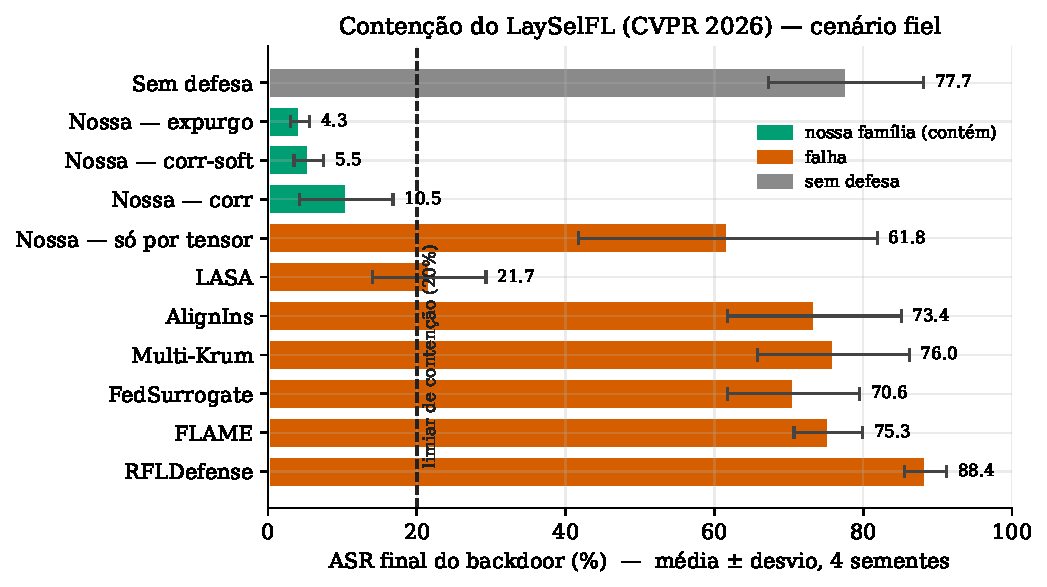
\includegraphics[width=\linewidth]{fig_rigor_asr.pdf}
  \caption{ASR final do backdoor no cenário fiel do LaySelFL (11 agregações, 4 sementes). Nossa
  família (verde) fica muito abaixo do limiar de contenção de 20\%; todas as defesas publicadas
  (laranja) falham. ``Nossa --- só por tensor'' mostra que agir tensor a tensor, sem corroborar,
  não basta.}
  \label{fig:rigor}
\end{figure}

\begin{table}[t]\centering\small
\caption{ASR final do backdoor, cenário fiel do LaySelFL, 11 agregações $\times$ 4 sementes.}
\label{tab:rigor}
\begin{tabular}{lcc}
\toprule
Agregação & ASR (4 sementes) & Contém? \\
\midrule
Sem defesa (referência) & $77{,}7\pm10{,}4\%$ & --- (ataque se fixa) \\
\textbf{Nossa --- expurgo do cliente} & $\mathbf{4{,}3\pm1{,}3\%}$ & sim \\
\textbf{Nossa --- consenso (corr-soft)} & $\mathbf{5{,}5\pm2{,}0\%}$ & sim \\
\textbf{Nossa --- corte por tensor (corr)} & $\mathbf{10{,}5\pm6{,}3\%}$ & sim (3/4) \\
Nossa --- apenas por tensor (sn) & $61{,}8\pm20{,}1\%$ & não \\
LASA & $21{,}7\pm7{,}6\%$ & não \\
AlignIns & $73{,}4\pm11{,}7\%$ & não \\
Multi-Krum & $76{,}0\pm10{,}2\%$ & não \\
FedSurrogate & $70{,}6\pm8{,}9\%$ & não \\
FLAME & $75{,}3\pm4{,}6\%$ & não \\
RFLDefense & $88{,}4\pm2{,}8\%$ & não \\
\bottomrule
\end{tabular}
\end{table}

\textbf{Generalidade.} A Fig.~\ref{fig:geral} estende o resultado a outras arquiteturas e ao
gatilho adaptativo. O ataque se fixa na VGG19 ($95{,}6\%$) e na EfficientNet ($85{,}3\%$); nossa
família contém na VGG19 ($9{,}2\%$, \emph{corr} $T{=}2$) e na EfficientNet ($13{,}0\%$,
\emph{corr-soft} $T{=}2$), confirmando a regra ``corroboração mais fraca $\Rightarrow$ expurgo mais
agressivo''.

\begin{figure}[t]\centering
  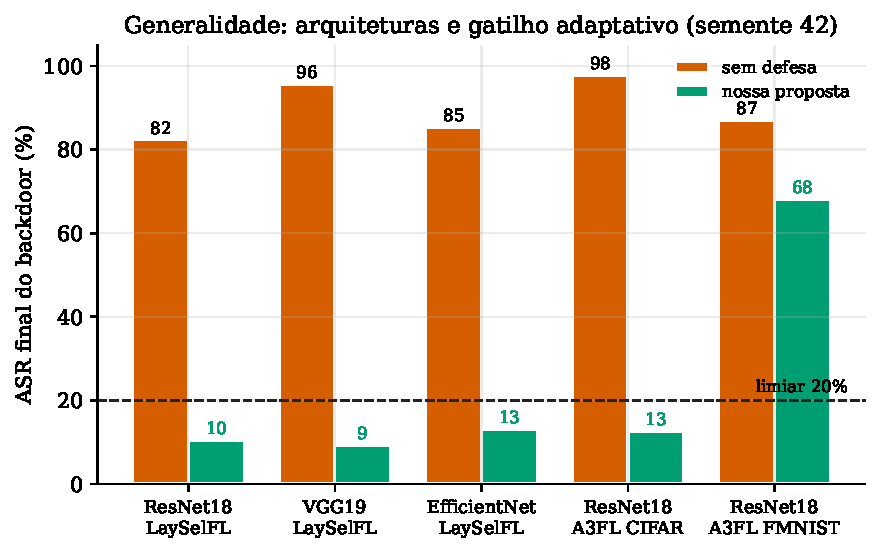
\includegraphics[width=\linewidth]{fig_generalidade.pdf}
  \caption{Generalidade (semente 42): ASR sem defesa (laranja) vs.\ nossa melhor variante (verde).
  A contenção se mantém em quatro dos cinco casos; a exceção (A3FL no FMNIST) é discutida na
  Seç.~\ref{sec:limits}.}
  \label{fig:geral}
\end{figure}

\textbf{Gatilho adaptativo (A3FL).} Sob o gatilho adversarialmente adaptativo A3FL \cite{a3fl}, o
ataque se fixa no CIFAR-10 ($97{,}7\%$) e nossa variante \emph{corr} o contém ($12{,}6\%$). O caso do
FMNIST ($68{,}2\%$) é uma assimetria conhecida sob investigação (Seç.~\ref{sec:limits}).

\textbf{Sobrecusto.} O agente adiciona $\leq 6{,}5\%$ de tempo por rodada em relação ao FedAvg
(Fig.~\ref{fig:overhead}), uma ordem de grandeza abaixo das defesas baseadas em busca
geométrica (LASA, AlignIns, RFLDefense), que chegam a $50$--$93\%$ na VGG19.

\begin{figure}[t]\centering
  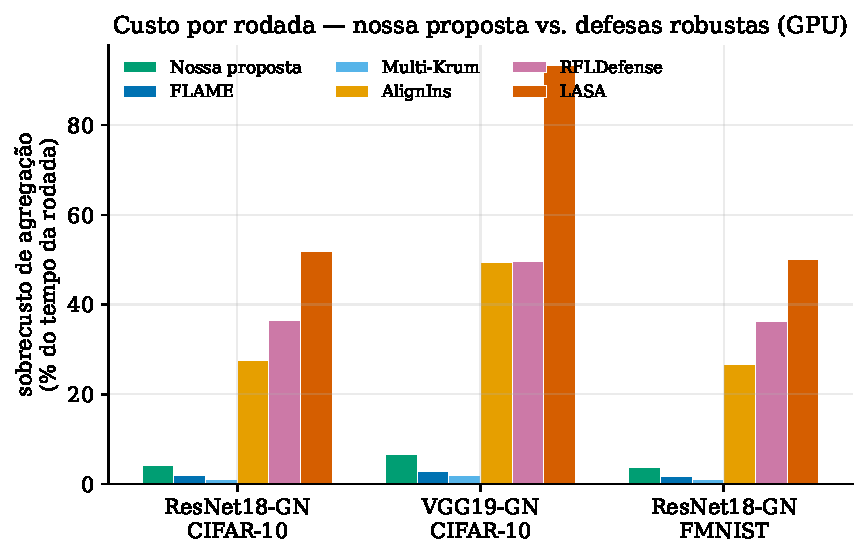
\includegraphics[width=\linewidth]{fig_overhead.pdf}
  \caption{Sobrecusto de agregação por rodada (\% do tempo de treino da rodada, em GPU). Nossa
  proposta fica junto das defesas mais baratas (FLAME, Multi-Krum) e muito abaixo das baseadas em
  busca geométrica.}
  \label{fig:overhead}
\end{figure}

\textbf{Sensibilidade ao limiar $T$.} Fixamos $T{=}8$ antes de rodar, a partir da curva de detecção
(Fig.~\ref{fig:curvaT}), medida sem retreinar o modelo. Para verificar se essa escolha depende de
ajuste fino, retreinamos a variante \emph{corr} com $T\in\{4,11,14\}$ nas sementes 42--44, sem mudar
mais nada (Tabela~\ref{tab:sensT}). Todos os valores testados reduzem o ataque de $83{,}2\%$ para
$11{,}5$--$17{,}1\%$ em média, o que confirma o patamar largo da curva de detecção. Os extremos
mostram os dois lados do compromisso: com $T{=}4$ o expurgo fica mais agressivo, custa $2{,}4$\,pp de
acurácia em relação a $T{=}8$ e, ainda assim, não contém a semente 44 ($28{,}3\%$); com $T{=}14$ a
detecção perde revocação e a ASR média sobe para $17{,}1\%$, com duas sementes perto do limiar de
$20\%$. O melhor resultado ficou em $T{=}11$ ($11{,}5\pm1{,}4\%$, contém nas 3 sementes), perto do
pico de $F_1$ da curva ($T{=}12$). Mantemos $T{=}8$, fixado antes, e reportamos a varredura como
evidência de que o resultado não depende de calibrar $T$ com o ataque conhecido.

\begin{table}[t]\centering\small
\caption{Sensibilidade ao limiar $T$ (variante \emph{corr}, cenário fiel do LaySelFL, sementes 42--44).
ASR final e acurácia final em \%; ``contém'' = ASR final $\leq 20\%$.}
\label{tab:sensT}
\begin{tabular}{lcccc}
\toprule
$T$ & ASR (s42 / s43 / s44) & ASR média & Contém & Acurácia \\
\midrule
4 & $5{,}9$ / $5{,}9$ / $28{,}3$ & $13{,}4\pm13{,}0$ & 2/3 & $70{,}8$ \\
\textbf{8 (fixado antes)} & $7{,}9$ / $7{,}6$ / $21{,}4$ & $12{,}3\pm7{,}9$ & 2/3 & $73{,}2$ \\
11 & $10{,}7$ / $10{,}7$ / $13{,}1$ & $11{,}5\pm1{,}4$ & 3/3 & $73{,}6$ \\
14 & $18{,}2$ / $19{,}9$ / $13{,}2$ & $17{,}1\pm3{,}5$ & 3/3 & $73{,}8$ \\
Sem defesa & $82{,}3$ / $78{,}1$ / $89{,}2$ & $83{,}2$ & 0/3 & $75{,}5$ \\
\bottomrule
\end{tabular}
\end{table}

\textbf{Custo sem ataque (falsos positivos).} Sob ataque, a precisão da detecção em $T{=}8$ é
$0{,}82$, ou seja, alguns honestos também são confirmados. Para medir o custo disso, repetimos o
cenário fiel com todos os 20 clientes honestos (mesma partição de dados, janela de ataque nunca
iniciada), em $\alpha{=}0{,}9$, o cenário do LaySelFL, e em $\alpha{=}0{,}1$, com dados muito mais
heterogêneos (Tabela~\ref{tab:fp}). Nenhuma variante cria backdoor: a ASR do gatilho fica em
$1{,}5$--$7{,}8\%$, o mesmo nível do modelo sem defesa ($6{,}1$--$6{,}7\%$). O custo de acurácia
separa as variantes. A \emph{corr-soft} é a mais barata ($-1{,}8$\,pp em $\alpha{=}0{,}9$ e $-3{,}0$\,pp
em $\alpha{=}0{,}1$), porque troca a contribuição suspeita pelo consenso em vez de descartá-la. A
\emph{client}, que descarta qualquer cliente acusado por um único tensor, retira em média 10 dos 20
clientes por avaliação e perde $5{,}2$\,pp em $\alpha{=}0{,}9$ e $13{,}8$\,pp em $\alpha{=}0{,}1$. Por
isso recomendamos a \emph{corr-soft} no caso geral e reservamos a \emph{client} para ameaça alta.

\begin{table}[t]\centering\small
\caption{Custo sem ataque (semente 42; 20 clientes honestos). Acurácia final em \%; $\Delta$ em
relação à agregação sem defesa; ``descartados'' = honestos confirmados por avaliação (média).}
\label{tab:fp}
\begin{tabular}{lcccc}
\toprule
& \multicolumn{2}{c}{$\alpha{=}0{,}9$} & \multicolumn{2}{c}{$\alpha{=}0{,}1$} \\
Agregação & Acurácia ($\Delta$) & Descartados & Acurácia ($\Delta$) & Descartados \\
\midrule
Sem defesa & $76{,}7$ & 0 & $67{,}9$ & 0 \\
\textbf{corr-soft} & $74{,}8$ ($-1{,}8$) & $1{,}6$ & $64{,}9$ ($-3{,}0$) & $2{,}8$ \\
corr & $74{,}5$ ($-2{,}2$) & $2{,}0$ & $63{,}8$ ($-4{,}2$) & $3{,}2$ \\
client & $71{,}5$ ($-5{,}2$) & $10{,}2$ & $54{,}2$ ($-13{,}8$) & $7{,}8$ \\
\bottomrule
\end{tabular}
\end{table}

\textbf{CIFAR-100.} Repetimos o cenário fiel no CIFAR-100, com 100 classes, nas sementes 42 e 43
(Tabela~\ref{tab:c100}). O ataque se fixa ($33{,}4$ e $45{,}0\%$ de ASR final; picos de $51$ a $58\%$)
e as três variantes o contêm por completo ($0{,}0$--$0{,}2\%$ de ASR final, pico máximo de $1{,}2\%$).
A acurácia do modelo limpo, treinado sem ataque e sem defesa, é $44{,}6\%$; a \emph{corr} e a
\emph{corr-soft} perdem de $2{,}3$ a $3{,}1$\,pp em relação à agregação sem defesa, e a \emph{client}
perde $6{,}7$ a $11{,}4$\,pp. Ao contrário do CIFAR-10, aqui a LASA também contém ($0{,}1$--$0{,}2\%$),
com custo semelhante ao nosso; FedSurrogate ($34$--$44\%$) e FLAME ($57$--$69\%$) falham. O CIFAR-100,
portanto, mostra que a contenção se mantém com muitas classes, mas não diferencia a nossa proposta
da LASA; a diferença entre as duas está no CIFAR-10, onde a LASA contém em apenas 2 de 6 sementes.

\begin{table}[t]\centering\small
\caption{CIFAR-100, cenário fiel (ResNet18-GN, 20 clientes, 6 maliciosos), sementes 42 e 43. Valores
em \%. Modelo limpo (sem ataque): acurácia $44{,}6\%$, ASR do gatilho $0{,}1\%$.}
\label{tab:c100}
\begin{tabular}{lccc}
\toprule
Agregação & ASR final (s42 / s43) & Pico da ASR & Acurácia \\
\midrule
Sem defesa & $33{,}4$ / $45{,}0$ & $51{,}1$ / $57{,}7$ & $43{,}3$ / $44{,}8$ \\
\textbf{corr-soft} & $0{,}2$ / $0{,}1$ & $0{,}3$ / $0{,}4$ & $40{,}2$ / $42{,}0$ \\
\textbf{corr} & $0{,}2$ / $0{,}2$ & $0{,}2$ / $0{,}6$ & $40{,}6$ / $42{,}5$ \\
\textbf{client} & $0{,}0$ / $0{,}2$ & $0{,}2$ / $1{,}2$ & $31{,}9$ / $38{,}1$ \\
LASA & $0{,}2$ / $0{,}1$ & $0{,}2$ / $0{,}3$ & $40{,}9$ / $42{,}8$ \\
FedSurrogate & $34{,}1$ / $43{,}5$ & $49{,}3$ / $59{,}9$ & $43{,}0$ / $44{,}5$ \\
FLAME & $57{,}0$ / $68{,}8$ & $75{,}3$ / $83{,}7$ & $37{,}0$ / $38{,}1$ \\
\bottomrule
\end{tabular}
\end{table}
